\section{Installation Packages}

\begin{frame}{\secname}

  \begin{columns}
    \begin{column}{.3\textwidth}
      \centering
      Official: \smallskip

      \faWindows\ Installer/Updater \\
      \faWindows\ Portable *.zip \\
      \faApple\ Installer/Updater \\
      \faApple\ Portable *.dmg \\
      \faLinux\ Installer/Updater \\
      \faLinux\ Portable *.tar.gz \\
      \faLinux\ Portable AppImage \\
      {\bfseries\faLinux\ Flatpak on Flathub} \\
      {\bfseries\faLinux\ Snap on Snapcraft} \\
    \end{column}

    \begin{column}{.6\textwidth}
      \centering
      \faRocket \hspace{0.05em} Community maintained: \smallskip

      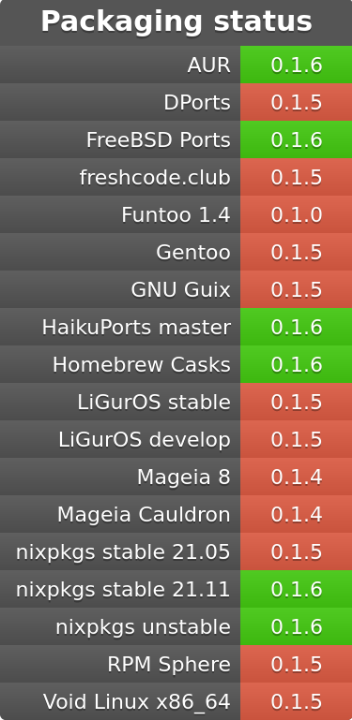
\includegraphics[height=6cm]{images/packaging_status.png}

      \ldots and even more!
    \end{column}
  \end{columns}

\end{frame}

\note{
  Now, let's take a look at things happened within the last two years
  beside the new features.\\

  One cool thing is that the number of installation packages is constantly
  increasing. Beside our official installers and portable packages we provide
  since the first release, LibrePCB is now also available as a Flatpak and as
  a Snap package.\\

  In addition, the community packages LibrePCB for many different distributions,
  for example Arch linux, FreeBSD, NixOS, and so on. That's pretty cool, thanks
  a lot to the package maintainters!
}

\begin{frame}{\secname}
  LibrePCB in Ubuntu Software:
  \begin{center}
    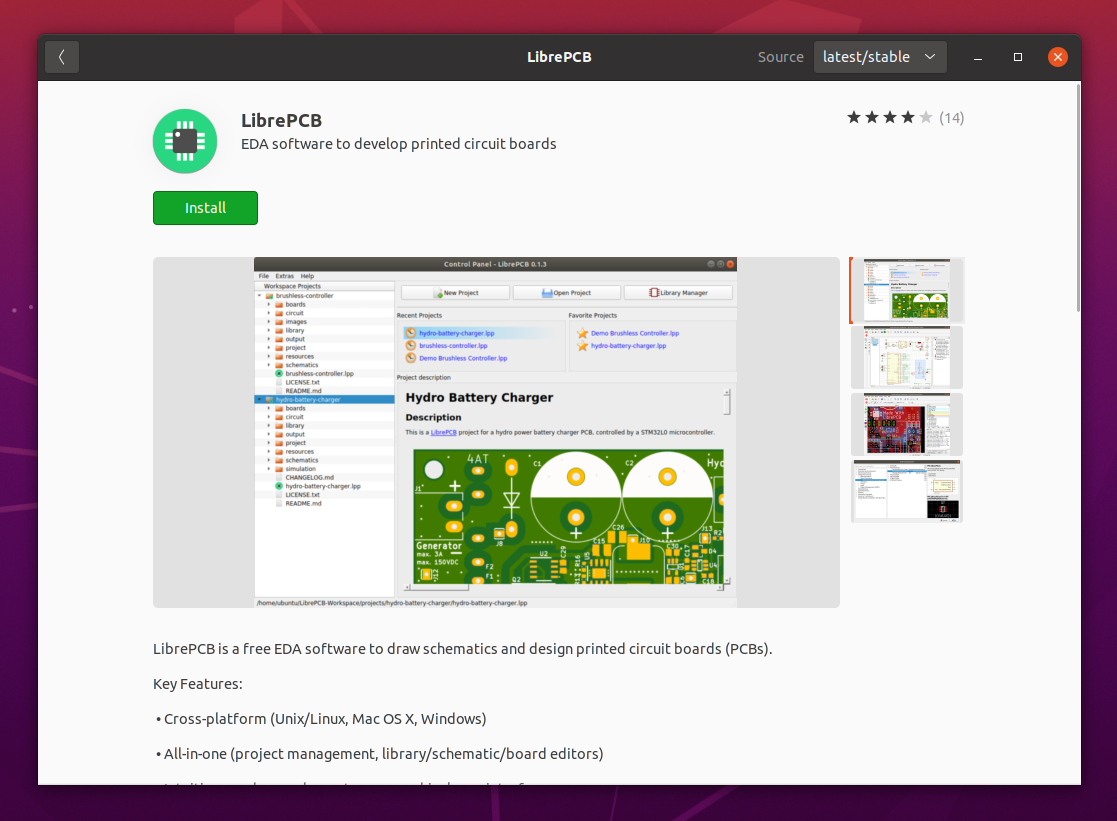
\includegraphics[height=6.3cm]{images/ubuntu_store.png}
  \end{center}
\end{frame}

\note{
  Due to the Snap package on Snapcraft, LibrePCB is now even available out of
  the box in the Ubuntu Software center.
}
